%%%%%%%%%%%%%%%%%%%%%%%%%%%%%%%%%%%%%%%%%
% Jacobs Landscape Poster
% LaTeX Template
% Version 1.0 (29/03/13)
%
% Created by:
% Computational Physics and Biophysics Group, Jacobs University
% https://teamwork.jacobs-university.de:8443/confluence/display/CoPandBiG/LaTeX+Poster
% 
% Further modified by:
% Nathaniel Johnston (nathaniel@njohnston.ca)
%
% This template has been downloaded from:
% http://www.LaTeXTemplates.com
%
% License:
% CC BY-NC-SA 3.0 (http://creativecommons.org/licenses/by-nc-sa/3.0/)
%
%%%%%%%%%%%%%%%%%%%%%%%%%%%%%%%%%%%%%%%%%

%----------------------------------------------------------------------------------------
%	PACKAGES AND OTHER DOCUMENT CONFIGURATIONS
%----------------------------------------------------------------------------------------

\documentclass[final]{beamer}
\usepackage[scale=0.78,size=a1]{beamerposter} % Use the beamerposter package for laying out the poster
% \usepackage[size=ansiD]{beamerposter} % Use the beamerposter package for laying out the poster

\usetheme{confposter} % Use the confposter theme supplied with this template

\setbeamercolor{block title}{fg=ngreen,bg=white} % Colors of the block titles
\setbeamercolor{block body}{fg=black,bg=white} % Colors of the body of blocks
\setbeamercolor{block alerted title}{fg=white,bg=dblue!70} % Colors of the highlighted block titles
\setbeamercolor{block alerted body}{fg=black,bg=dblue!10} % Colors of the body of highlighted blocks
% Many more colors are available for use in beamerthemeconfposter.sty

%-----------------------------------------------------------
% Define the column widths and overall poster size
% To set effective sepwid, onecolwid and twocolwid values, first choose how many columns you want and how much separation you want between columns
% In this template, the separation width chosen is 0.024 of the paper width and a 4-column layout
% onecolwid should therefore be (1-(# of columns+1)*sepwid)/# of columns e.g. (1-(4+1)*0.024)/4 = 0.22
% Set twocolwid to be (2*onecolwid)+sepwid = 0.464
% Set threecolwid to be (3*onecolwid)+2*sepwid = 0.708

\newlength{\sepwid}
\newlength{\onecolwid}
\newlength{\twocolwid}
\newlength{\threecolwid}
% \setlength{\paperwidth}{33.1in} % A0 width: 46.8in
% \setlength{\paperheight}{23.4in} % A0 height: 33.1in
\setlength{\paperwidth}{34in} % A0 width: 46.8in
\setlength{\paperheight}{22in} % A0 height: 33.1in
\setlength{\sepwid}{0.024\paperwidth} % Separation width (white space) between columns
\setlength{\onecolwid}{0.22\paperwidth} % Width of one column
\setlength{\twocolwid}{0.464\paperwidth} % Width of two columns
\setlength{\threecolwid}{0.708\paperwidth} % Width of three columns
\setlength{\topmargin}{-0.5in} % Reduce the top margin size
%-----------------------------------------------------------

\usepackage{graphicx}  % Required for including images

\usepackage{booktabs} % Top and bottom rules for tables

\usepackage{braket,subcaption}

%----------------------------------------------------------------------------------------
%	TITLE SECTION 
%----------------------------------------------------------------------------------------

\title{Numerical Time-Dependent Schr\"{o}dinger Equation} % Poster title

\author{John Doherty and Ricardo Castro Yarza} % Author(s)

\institute{University of Illinois at Urbana-Champaign\\Deptartment of Computer Science and Department of Physics} % Institution(s)

%----------------------------------------------------------------------------------------

\begin{document}

\addtobeamertemplate{block end}{}{\vspace*{2ex}} % White space under blocks
\addtobeamertemplate{block alerted end}{}{\vspace*{2ex}} % White space under highlighted (alert) blocks

\setlength{\belowcaptionskip}{2ex} % White space under figures
\setlength\belowdisplayshortskip{2ex} % White space under equations

\begin{frame}[t] % The whole poster is enclosed in one beamer frame

\begin{columns}[t] % The whole poster consists of three major columns, the second of which is split into two columns twice - the [t] option aligns each column's content to the top

\begin{column}{\sepwid}\end{column} % Empty spacer column

\begin{column}{\onecolwid} % The first column

%----------------------------------------------------------------------------------------
%	OBJECTIVES
%----------------------------------------------------------------------------------------

\begin{alertblock}{Abstract}
The Time-Dependent Schr\"{o}dinger Equation (TDSE) describes the quantum state of a particle in the non relativistic regime. The lack of analytical solutions for most cases of interest motivates its study with numerical methods. We present a numerical scheme for the TDSE using the Finite Element Method and Crank-Nicolson.
\end{alertblock}

%----------------------------------------------------------------------------------------
%	INTRODUCTION
%----------------------------------------------------------------------------------------

\begin{block}{Introduction}
The TDSE is, in natural units ($\hbar=1$):
\begin{equation}
i\partial_{t}\ket{\psi}=\hat{H}\ket{\psi}
\end{equation}
and takes the following form in position basis:
\begin{equation}
i\partial_{t}\psi=\left[-\frac{1}{2m}\nabla^{2}+V\left(\mathbf{r}\right)\right]\psi
\label{SchrodPosBasis}
\end{equation}
The probability density for the particle's position is given by:
\begin{equation}
\left|\psi\left(\mathbf{r},t\right)\right|^{2}
\end{equation}
\end{block}
\begin{block}{Numerical method}
Due to its geometric flexibility, finite element method with quadratic elements was preferred. The chosen timestepping method is Crank-Nicolson because it is unitary, meaning the norm of the solution is preserved and thus is probability. Applying these two methods requires computing the potential-weighted mass matrix, $C$, given by:
\begin{equation}
C_{ij} = \int\phi_{i}\phi_{j}V\left(\mathbf{r}\right)\,\mathrm{d}\mathbf{x}
\end{equation}
In terms of the global finite element matrices $A$ (stiffness), $B$ (mass), and potential-weighted mass $C$, the timestepping operator (equivalent to the quantum mechanical propagator in the position basis) is:
	%\begin{equation}
	%iv_{i}\left(\int\phi_{i}\phi_{j}\,\mathrm{d}\mathbf{x}\right)\dot{\psi}_{j}=\frac{1}{2m}v_{i}\left(\int\nabla\phi_{i}\nabla\phi_{j}\,\mathrm{d}\mathbf{x}\right)\dot{\psi}_{j}
	%\end{equation}
\begin{equation}
U=\left[B+\frac{i\Delta t}{2}\left(\frac{A}{2m}+C\right)\right]^{-1}\left[B-\frac{i\Delta t}{2}\left(\frac{A}{2m}-C\right)\right]
\end{equation}
which satisfies:
\begin{equation}
\psi^{n+1}=U\psi^{n}
\end{equation}
\end{block}

%----------------------------------------------------------------------------------------

%----------------------------------------------------------------------------------------
%----------------------------------------------------------------------------------------

\end{column} % End of the first column

\begin{column}{\sepwid}\end{column} % Empty spacer column

\begin{column}{\twocolwid} % Begin a column which is two columns wide (column 2)

\begin{columns}[t,totalwidth=\twocolwid] % Split up the two columns wide column

\begin{column}{\onecolwid}\vspace{-.6in} % The first column within column 2 (column 2.1)

%----------------------------------------------------------------------------------------
%	ALGORITHM
%----------------------------------------------------------------------------------------
%\begin{block}{Problem descriptions}
%The problem to solve is the 2D TDSE (equation \eqref{SchrodPosBasis}) for the double slit experiment with the following restrictions:
%	\begin{gather}
%	V=0,\quad\Omega=\left[0,1\right]^{2},\quad\psi = 0\text{ on } \partial\Omega
%	\end{gather}
%	for a variety of initial conditions.
%\end{block}
\begin{block}{Test case}
The test problem is the 2D infinite square well, defined by:
\begin{gather}
V=0,\quad\Omega=\left[0,1\right]^{2},\quad\psi = 0\text{ on } \partial\Omega
\end{gather}
This has an analytical solution, given an initial wavefunction, which is shown below. The initial wavefunction used was a superposition of two eigenstates, $n_x=1$, $n_y=1$ and $n_x=2$, $n_y=2$.

\begin{gather}
E_n = \frac{\pi^2}{2 m l_x l_y}(n_x^2 + n_y^2)
\end{gather}
\begin{gather}
\psi(x,y,t) = \sum_{n_x, n_y} \frac{1}{4} \frac{\sqrt{2}}{l_x} \frac{\sqrt{2}}{l_y} \sin(n_x \pi x) \sin(n_y \pi y) e^{-i E_n }
\end{gather}

\begin{figure}[H]
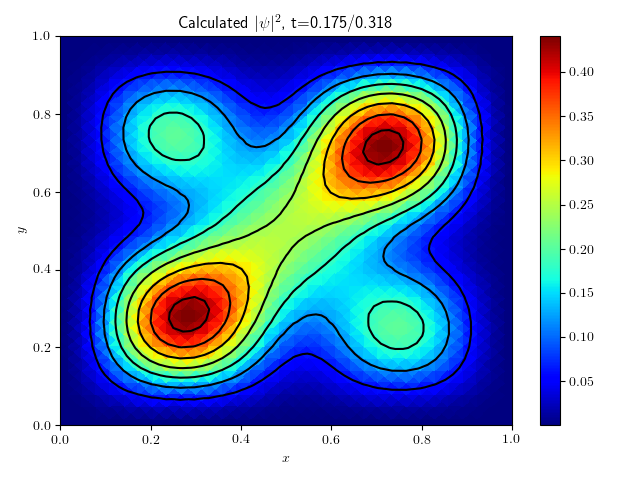
\includegraphics[width=\linewidth]{toy_sol.png}
\caption{Graph of the calculated probability distribution.}
\end{figure}

%The error measurements taken were of the relative infinity norm at $t_f=\frac{1}{\pi}$. This is:
%\begin{equation}
%\epsilon=\frac{\left|\left|\psi-\tilde{\psi}\right|\right|_{\infty}}{\left|\left|\tilde{\psi}\right|\right|_{\infty}}
%\end{equation}
The error measurements taken were of the relative infinity norm at $t_f=\frac{1}{\pi}$. The estimated algebraic convergence rate is $2$ in $\Delta t$ and $3$ in $\Delta x$. This is expected because Crank-Nicolson is second order in time and quadratic basis functions are used.
 
\begin{table}
	\centering
	\begin{subtable}{.5\textwidth}
		\centering
		\begin{tabular}{c c}\toprule
			\textbf{Grid $\Delta x$} & \textbf{Error} \\\midrule
			2.5   \times 10^{-1} & 5.73 \times 10^{-2} \\
			6.25  \times 10^{-2} & 9.00 \times 10^{-4} \\
			3.125 \times 10^{-2} & 1.28 \times 10^{-4} \\\bottomrule
		\end{tabular}
				%\caption{Relative Error at $t_f = \frac{1}{\pi}$}
	\end{subtable}%
	\begin{subtable}{.5\textwidth}
		\centering
		\begin{tabular}{c c}\toprule
			\textbf{Timestep $\Delta t$} & \textbf{Error} \\\midrule
			3.18 \times 10^{-2} & 2.54 \times 10^{-1} \\
			3.18 \times 10^{-3} & 6.02 \times 10^{-3} \\
			3.18 \times 10^{-4} & 1.32 \times 10^{-4} \\\bottomrule
		\end{tabular}
				%\caption{Relative Error at $t_f = \frac{1}{\pi}$}
	\end{subtable}
		\caption{Summary of convergence properties.}
\end{table}
\end{block}

%----------------------------------------------------------------------------------------

\end{column} % End of column 2.1

\begin{column}{\onecolwid}\vspace{-.6in} % The second column within column 2 (column 2.2)

%----------------------------------------------------------------------------------------
%	METHODS
%----------------------------------------------------------------------------------------

\begin{block}{Double slit experiment}
The domain is similar to $\Omega=[-1,1]^{2}$ with a division at $x=0$ and two slits at around $y=0$ connecting the two halves. $V=0$ with homogeneous Dirichlet boundary conditions and a plane wave initial condition $e^{ikx}$%$\exp\left(ikx\right)$.
\begin{figure}[H]
\includegraphics[width=\linewidth]{DoubleSlit0.png}
\caption{Initial conditions for double slit.}
\end{figure}
The wave travels to the right and hits the slits. A part is reflected, and the transmitted one experiences interference:
\begin{figure}[H]
	\includegraphics[width=\linewidth]{DoubleSlit115.png}
	\caption{Double slit solution.}
\end{figure}
\end{block}

%----------------------------------------------------------------------------------------

\end{column} % End of column 2.2

\end{columns} % End of the split of column 2 - any content after this will now take up 2 columns width

%----------------------------------------------------------------------------------------
%	IMPORTANT RESULT
%----------------------------------------------------------------------------------------

% \begin{alertblock}{Important Result}

% Lorem ipsum dolor \textbf{sit amet}, consectetur adipiscing elit. Sed commodo molestie porta. Sed ultrices scelerisque sapien ac commodo. Donec ut volutpat elit.

% \end{alertblock} 

%----------------------------------------------------------------------------------------

\begin{columns}[t,totalwidth=\twocolwid] % Split up the two columns wide column again

% \begin{column}{\onecolwid} % The first column within column 2 (column 2.1)

% %----------------------------------------------------------------------------------------
% %	MATHEMATICAL SECTION
% %----------------------------------------------------------------------------------------

% % \begin{block}{Multilevel RSB Algorithm}

% % \begin{itemize}
% % 	\item 4 steps.
% % \end{itemize}

% % % \begin{equation}
% % % E = mc^{2}
% % % \label{eqn:Einstein}
% % % \end{equation}

% % \end{block}

% %----------------------------------------------------------------------------------------

% \end{column} % End of column 2.1

% \begin{column}{\onecolwid} % The second column within column 2 (column 2.2)

%----------------------------------------------------------------------------------------
%	RESULTS
%----------------------------------------------------------------------------------------

% \begin{block}{Current status}

% \begin{center}
% \begin{tabular}{cc}
% \includegraphics[width=0.4\linewidth]{mesh_1.png} & \hfill & \includegraphics[width=0.4\linewidth]{mesh_2.png}
% \end{tabular}
% \end{center}

%  \end{block}

%----------------------------------------------------------------------------------------



% \end{column} % End of column 2.2

\end{columns} % End of the split of column 2

\end{column} % End of the second column

\begin{column}{\sepwid}\end{column} % Empty spacer column

\begin{column}{\onecolwid} % The third column

%----------------------------------------------------------------------------------------
%	CONCLUSION
%----------------------------------------------------------------------------------------
\begin{block}{}
	Classically, the expected result is to detect particles in regions with the same shape as the slits, but this does not happen. This shows the inability to explain properties of quantum-scale objects by considering them as exclusively particles or waves, and leads to the concept of wave-particle duality.
	
\end{block}
\begin{block}{Conclusion}
A numerical realization of the double slit experiment was presented, showing that the Time-Dependent Schr\"{o}dinger equation predicts wave-like behavior for objects in the quantum scale.\par
It was also shown that Crank-Nicolson is a reasonable timestepping scheme for this problem based on the error statistics and the conservation of probability.

\end{block}

%----------------------------------------------------------------------------------------
%	ADDITIONAL INFORMATION
%----------------------------------------------------------------------------------------

\begin{block}{Future Work}
In order to address many systems of physical importance, the current work could be modified to make a general solver for the TDSE. This process involves the following:
\begin{itemize}
\item Generalize boundary conditions.
\item Improve spatial resolution.
\item Use time-dependent potentials.
\item Implement in 3D.
\end{itemize}

\end{block}

%----------------------------------------------------------------------------------------
%	REFERENCES
%----------------------------------------------------------------------------------------

\begin{block}{References}

\nocite{*} % Insert publications even if they are not cited in the poster
\small{\bibliographystyle{unsrt}
\bibliography{bib.bib}\vspace{0.75in}}

\end{block}

%----------------------------------------------------------------------------------------
%	ACKNOWLEDGEMENTS
%----------------------------------------------------------------------------------------

% \setbeamercolor{block title}{fg=red,bg=white} % Change the block title color

% \begin{block}{Acknowledgements}

% \small{\rmfamily{Nam mollis tristique neque eu luctus. Suspendisse rutrum congue nisi sed convallis. Aenean id neque dolor. Pellentesque habitant morbi tristique senectus et netus et malesuada fames ac turpis egestas.}} \\

% \end{block}

%----------------------------------------------------------------------------------------
%	CONTACT INFORMATION
%----------------------------------------------------------------------------------------

% \setbeamercolor{block alerted title}{fg=black,bg=norange} % Change the alert block title colors
% \setbeamercolor{block alerted body}{fg=black,bg=white} % Change the alert block body colors

% \begin{alertblock}{Contact Information}

% \begin{itemize}
% \item Web: \href{http://www.university.edu/smithlab}{http://www.university.edu/smithlab}
% \item Email: \href{mailto:john@smith.com}{john@smith.com}
% \item Phone: +1 (000) 111 1111
% \end{itemize}

% \end{alertblock}

% \begin{center}
% \begin{tabular}{ccc}
% \includegraphics[width=0.4\linewidth]{logo.png} & \hfill & \includegraphics[width=0.4\linewidth]{logo.png}
% \end{tabular}
% \end{center}

%----------------------------------------------------------------------------------------

\end{column} % End of the third column

\end{columns} % End of all the columns in the poster

\end{frame} % End of the enclosing frame

\end{document}
